\section{Предложенные модификации}

В ходе анализа существующих методов и средств, направленных на ускорение получения модели алгоритмом ПЭГ и повышение её качества, а также проведённых экспериментов был выявлен ряд ограничений производительности алгоритма, таких как длительность вычисления фитнеса, отсутствие тонкой подстройки числовых констант, вляние размера хромосомы на скорость сходимости, проблемы с поиском сложных моделей. Далее описаны методы и подходы, созданные в ходе преодоления данных ограничений.

%--------------------------------------------------------------------

\subsection{Создание начальной популяции}

В изученных работах, посвящённых ПЭГ, не уделяется внимания процедуре создания начальной популяции, а именно конструированию случайной особи. Указывается, что строка хромосомы обходится с начала и по порядку, и каждый символ задаётся случайным образом: тип узла может быть равновероятно задан как функциональный элемент, как переменная (подаваемая на вход модели) и как числовая константа. Очевидно, что размер дерева определяется количеством подряд (близко) идущих функциональных узлов, начиная с корневого узла (первого символа хромосомы): из условия равновероятности типов узлов (3 типа~--- 33.333\%~каждый) следует, что вероятность создания дерева, состоящего всего из одного элемента (терминала: переменной либо константы), составляет~66.67\%. При этом можно заметить, что средняя длина получаемых деревьев не зависит от задаваемой длины хромосомы, но определяется установленной вероятностью появления того или иного типа.

При оригинальном кодировании элементов путём обхода узлов дерева в ширину логично предположить, что вероятность появления функциональных узлов в головной части хромосомы следует повысить, в то время как в хвостовой части могут быть помещены исключительно терминальные узлы. В таком случае определение оптимальных численных значений вероятностей представляет собой отдельную задачу для исследования. Кроме того, данный подход не применим к другим способам кодирования, потому не обладает должной универсальностью.

Для решения указанной проблемы и закрепления взаимосвязи между размером дерева и длиной генома была разработана следующая процедура инициализации. Обход строки так же производится посимвольно, начиная с её начала (независимо от способа кодирования). При этом не составляет трудности определить местонахождение кодируемого символом узла в дереве, а именно его глубину: первый символ является корневым узлом, далее~--- в соответствии со способом кодирования.

Вырожденное дерево, состоящее из одного терминала, как правило, не представляет интереса, так как решаемая таким образом задача не требует применения ПЭГ. В таком случае вероятность задания функционального типа корневому узлу устанавливается равным~100\%. В тоже время для ограничения размера дерева заданным значением (несмотря на способность префиксного кодирования и ПЭГ с наложениями создания деревьев, превышающих в размере длину генома) в целях удобства пользования уместно ограничить узлы максимальной возможной глубины листовыми. Следовательно, вероятность появления функционала в указанных местах равна нулю. Требует решения задача распределения вероятности функциональных узлов в зависимости от глубины вложенности.

Предлагается использование следующей формулы:

\begin{equation}
\label{eq:init_func_prob}
P_{func}(level, maxlevel) = \sqrt{1 - \left(\frac{level - 1}{maxlevel - 1}\right)^2}
\end{equation}

где $level$~--- глубина узла, $maxlevel$~--- максимально возможная глубина дерева. Пример такого распределения показан на рисунке~\ref{img:init_func_prob}.

\begin{figure} [h]
  \center
  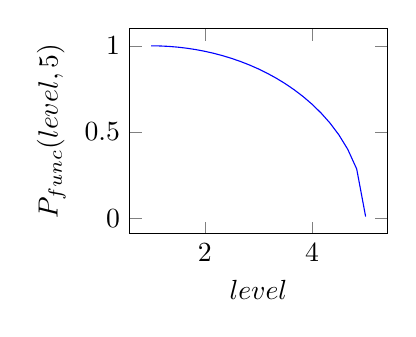
\begin{tikzpicture}[domain=1:5]
  	\begin{axis}[xlabel={$level$}, ylabel={$P_{func}(level, 5)$}, width=0.4\linewidth, no marks]
      \addplot{sqrt(1 - ((x - 1) / (5 - 1))^2)};
    \end{axis}
  \end{tikzpicture}
  \caption{Вероятность появления функционального узла в зависимости от глубины узла в дереве глубиной 5}
  \label{img:init_func_prob}
\end{figure}

Таким образом, процедура инициализации задает узлу глубины~$level$ тип функции при выполнении условия $random(0\ldots1) < P_{func}(level, maxlevel)$, обеспечивая сбалансированную начальную популяцию особей прогнозируемого размера. Данный метод конструирования новой особи случайным образом показал свою эффективность и был использован во всех экспериментах.

%--------------------------------------------------------------------

\subsection{Плавно-динамические константы}

Недостатком изученных операторов мутации численных констант является отсутствие тонкой подстройки коэффциентов особей: степень изменения ничем не ограничена, не предоставляя гарантий поступательного движения в сторону оптимума. Для направления процесса эволюции была построена следующая процедура, комбинирующая динамический подход работы с константами ПЭГ и метод иммунных сетей. Создание нового терминала-константы выполняется согласно динамическому подходу: новому узлу (при создании начальной популяции, либо после изменения типа узла на терминал-константу оператором мутации) задаётся значение одно из элементов массива <<золотых сечений>>~$A$. Оператор плавно-динамической мутации констант изменяет значение в пределах~$\pm10\%$ от текущего:

\begin{equation}
\label{eq:zerg_const_mutation}
V = V \times (1 + random(-0.1\ldots0.1))
\end{equation}

В показанной выше таблице~\ref{tbl:cmp_dynamic_mutation} продемонстрировано преимущество в эффективности такого подхода по сравнению с неограниченной мутацией. Данный оператор инициализации и мутации численных констант был использован во всех представленных экспериментах.

%--------------------------------------------------------------------

\subsection{Дополнительная популяция}

В качестве одной из мер повышения вероятности обнаружения решения было предложено использование дополнительной параллельной независимой популяции. Если при очередной итерации (поколении) работы алгоритма фитнес лучшей особи дополнительной популяции превысит фитнес лучшей особи основной популяции~--- данная особь копируется на место худшей особи основной популяции. Из результатов, представленных в таблице~\ref{tbl:cmp_add_pop} можно сделать вывод об успешном решении поставленной задачи при использовании данного подхода. Негативным следствием является снижение точности наилучшей из получаемых моделей. Это происходит по причине возрастания вычислений в расчёте на итерацию алгоритма, следовательно при равном отводимом времени работы модифицированный алгоритм успеет расчитать меньшее количество поколений.

\input{cmp_add_pop}

%--------------------------------------------------------------------

\subsection{Инкрементальная эволюция}

В приведённых выше таблицах~\ref{tbl:cmp_chrom_sizes} и~\ref{tbl:cmp_probability_density_selection_and_tournament} отчётливо заметно наличие некоторого оптимального размера генома, при котором достигается максимум производительности алгоритма. Данный размер требует отдельного определения для каждой задачи и каждого способа кодирования, для его выбора могут применяться как простой перебор параметров, так и описанные выше популяции неоднородных особей.

Более эффективным показал себя метод инкрементальной эволюции, в ходе которого производится ряд последовательных запусков алгоритма с наращиванием длины хромосомы при каждом запуске и копированием лучшей особи предыдущего запуска в начальную популяцию текущего. Такой подход требует меньших вычислительных ресурсов по сравнению с независимыми запусками, т.к. позволяет производить постепенное усложнение дерева. Результаты работы данной модификации приведены в таблице~\ref{tbl:cmp_incremental}.

\input{cmp_incremental}

%--------------------------------------------------------------------

\subsection{Частичный подсчёт фитнеса}
\cite{ferreira:2001:wsc6Aa}
Главным недостатком как эволюционных алгоритмов в целом, так и ПЭГ в частности~--- это их низкая скорость работы (по сравнению со скоростью посторения ИНН, регрессионных моделей). Любое ускорение алгоритма ПЭГ позволяет улучшить качество получаемых моделей по причине возможности произвести расчёт б\'{о}льшего количества поколений и выполнить больше независимых запусков за эквивалентное время.

Наиболее ресурсоёмкой частью алгоритма является вычисление фитнеса: на вход модели подаются все точки входных данных, которые затем обрабатываются в соответствии с программой (формулой, правилом), закодированной моделью. В ходе исследований, направленных на ускорение процедуры расчёта фитнеса, удалось получить универсальный метод, позволивший значительно улучшить оба показателя эффективности: как~$e_{b}$, так и~$r_{f}$.

В формулу расчёта фитнеса как правило входит СКО модели, а само значение фитнеса служит для сравнения эффективности моделей между собой. Было обнаружено, что для такой оценки не требуется вычисление СКО по полному набору подаваемых на вход данных. Если на определённом этапе текущее значение СКО (либо соответствующий фитнес) превысит некоторый порог~$threshold$~--- дальнейшие расчёты могут быть прерваны. Такой подход позволяет избежать лишних затрат на точное вычисление фитнеса плохо приспособленных особей, заменяя его приближённым оценочным значением.

Весь набор входных данных~$DataIn$ перемешивается для избежания последовательностей соседних точек, и разбивается на $G$~пакетов~$Dg_{k}$:

\begin{equation}
\label{eq:zerg_partial_mse_groups}
DataIn=\bigcup_{j=1\ldots G}{Dg_{j}}
\end{equation}

После обработки каждого пакета производится оценка фитнеса, и на её основании выносится решение о прерывании вычислений особи. Условием прерывания служит сравнение фитнеса по вычисленным первым~$K$ группам с пороговым значением~$threshold$, которое динамически изменяется в процессе эволюции и потому задаётся некоторой долей (например,~0.7) от среднего фитнеса популяции на предыдущем поколении:

\begin{equation}
\label{eq:zerg_partial_mse_fit_form}
f(i, g + 1) = f_{z}(i, 0.7 \frac{1}{N}\sum\limits_{j=1}^{N}{f(j,g)})
\end{equation}

\begin{equation}
\label{eq:zerg_partial_mse_fit_form_exp}
f_{p}(i, K) = f_{MSE}(i, \bigcup_{j=1\ldots K}{Dg_{j}}), K \le G
\end{equation}

где $f(i, g + 1)$, $f(i, g)$~--- возвращаемое значение фитнеса~$i$-той особи расчитываемого и предыдущего поколений, $f_{z}(i, threshold)$~--- функция взвешенного фитнеса, $N$~--- размер популяции, $K$~--- количество обработанных групп входных данных. Для того, чтобы внести различие между особями, расчёт которых был прерван в различные моменты времени (пороговое значение ошибки было превышено при разном количестве обработанных групп входных данных), был добавлен коэффициент штрафа~$K/G$:

\begin{equation}
\label{eq:zerg_partial_mse_fitness}
f_{z}(i, threshold) =
	\begin{cases}
		f_{p}(i, G) & f_{p}(i, G) \ge threshold \\
		f_{p}(i, K)\frac{K}{G} & f_{p}(i, K) < threshold
	\end{cases}
\end{equation}

Таким образом, плохие решения будут занимать меньшее количество ресурсов, в то время как лучшие особи будут вычислены наиболее точно. В таблице~\ref{tbl:cmp_partial_mse_r_squared} приведено сравнение производительности исходных алгоритмов с модифицированными частичным подсчётом СКО.

\input{cmp_partial_mse_r_squared}

%--------------------------------------------------------------------

%\subsection{Применение иммунных алгоритмов к оптимизации констант}

%--------------------------------------------------------------------

\subsection{Итеративный разностный подход}

Одна из наиболее распространённых задач, для решения которой применяется ПЭГ~--- поиск математической формулы, описывающей набор численных данных, этот процесс называется символьной регрессией, либо, в более простом варианте, аппроксимацией функций. Примером такой задачи может служить обнаружение формулы, описывающей сложную поверхность. В ряде случаев сложность моделируемого объекта такова, что обеспечить приемлемую точность при описании компактной формулой невозможно, и требуется увеличить размер искомого дерева, что приводит к резкому росту пространства поиска, а следовательно и вычислительного времени.

Популярным средством повышения сложности формулы с минимальным влиянием на производительность алгоритма является развитие идеи сложных мультигенных хромосом с иерархической структуров, которые были описаны выше.

Ещё более действенным показал себя разработанный в ходе данных исследований разностный подход, основанный на простоте комбинирования синтаксических деревьев: математические формулы могут быть легко объединены, например, при помощи функции арифметического сложения, правила классификаторов~--- булевыми <<И>> и <<ИЛИ>>, и т.д. Эта особенность позволяет составить сложную формулу из ряда простых, компактных и быстро вычисляемых по отдельности.

Суть подхода заключается в последовательном применении алгоритма ПЭГ с неизменным набором параметров к поверхностям ошибки~--- наборам численных данных, полученных путём вычитания очередной полученной модели из моделируемых данных. Тем самым разностных подход принципиально отличается от идеи эволюции мультигенных хромосом, где алгоритм пытается обнаружить решение с первой же итерации. При первом запуске на вход алгоритма ПЭГ подаётся набор данных~$T(O_{0})$, с ожиданием на выходе модели~$M$, возвращающей набор данных~$O$:

\begin{equation}
\label{eq:zerg_diff_m_1}
\{M_{1}, O_{1}\} = GEP(T = O_{0})
\end{equation}

На каждом следующем этапе на вход подаётся разность моделей:

\begin{equation}
\label{eq:zerg_diff_m_i}
\{M_{i+1}, O_{i+1}\} = GEP(O_{i} - O_{i - 1})
\end{equation}

Итоговой моделью после N запусков является:

\begin{equation}
\label{eq:zerg_diff_model}
M = M_{1} + M_{2} + \ldots + M_{N}
\end{equation}

В таблице~\ref{tbl:cmp_differential} показано сильнейшее положительное влияние разностного подхода на показатели алгоритма ПЭГ. Следует, однако, учитывать при этом возрастающее пропорционально количеству разностей время, затрачиваемое алгоритмом на поиск каждого слагаемого формулы модели.

\input{cmp_differential}